\documentclass[conference]{IEEEtran}
\IEEEoverridecommandlockouts
% The preceding line is only needed to identify funding in the first footnote. If that is unneeded, please comment it out.
\usepackage{cite}
\usepackage{amsmath,amssymb,amsfonts}
\usepackage{algorithmic}
\usepackage{graphicx}
\usepackage{url}
\usepackage[utf8]{inputenc}
\usepackage{textcomp}


\usepackage[english,ngerman,brazilian]{babel}
\def\BibTeX{{\rm B\kern-.05em{\sc i\kern-.025em b}\kern-.08em
    T\kern-.1667em\lower.7ex\hbox{E}\kern-.125emX}}
\begin{document}

\title{Projeto Demonstrativo 2 - Calibração de Câmeras}

\author{\IEEEauthorblockN{Frederico Guth (18/0081641)}
\IEEEauthorblockA{\textit{Tópicos em Sistemas de Computação, ,} \\
\textit{Turma TC - Visão Computacional (PPGI)}\\
\textit{Universidade de Brasília}\\
Brasília, Brasil\\
fredguth@fredguth.com}
}

\maketitle

\begin{abstract}
Uma câmera faz um mapeamento geométrico do mundo para uma imagem e é possível, fazer o caminho inverso, mapeando a posição de objetos no mundo a partir da sua imagem. Para isso, entretanto, é preciso conhecer os parâmetros intrínsecos e extrínsecos da câmera, o que chamamos de calibração. Neste projeto mostramos como calibrar a câmera e obter informações do mundo 3D a partir de imagens.
\end{abstract}

\begin{IEEEkeywords}
câmeras, calibração, parâmetros intrísecos, parâmetros extrínsecos, projeção reversa
\end{IEEEkeywords}

\section{Introdução}
Uma câmera faz um mapeamento geométrico do mundo 3D para o plano de uma imagem 2D. Conhecendo seus parâmetros intrínsecos, como distância focal e distorções da lente, e extrínsecos, sua rotação e translação no sistema de coordenadas do mundo real, é possível estimar a posição 3D de um objeto a partir de sua imagem\cite{tese}. 

Isto possibilita diversas aplicações: por exemplo, a mensuração da altura de pessoas registradas em vídeos de camêras de segurança ou a estimativas de posições de atletas em campo, entre outras.

\subsection{Objetivos}
Os objetivos deste projeto são a aplicação prática da teoria de calibração de câmeras e o desenvolvimento de uma "régua visual", capaz de medir um objeto através da sua imagem.

Mais especificamente deseja-se:
\begin{enumerate}
\item medir um segmento de reta em imagens através de cliques de mouse;
\item realizar a calibração de uma câmera digital, armazenando os parâmetros intrísecos e os coeficientes de distorções em arquivos XML;
\item realizar a calibração de uma câmera digital a partir de diferentes distâncias da câmera, calculando os parâmetros extrínsecos da mesma e avaliando a diferença dos resultados;
\item medir um objeto através de sua imagem e comparar com suas dimensões reais;
\item analisar os resultados obtidos.
\end{enumerate}
\section{Revisão Teórica}

\subsection{Câmera Estenopeica com Coordenadas Homogêneas}

\begin{figure}[ht!]
\begin{center}
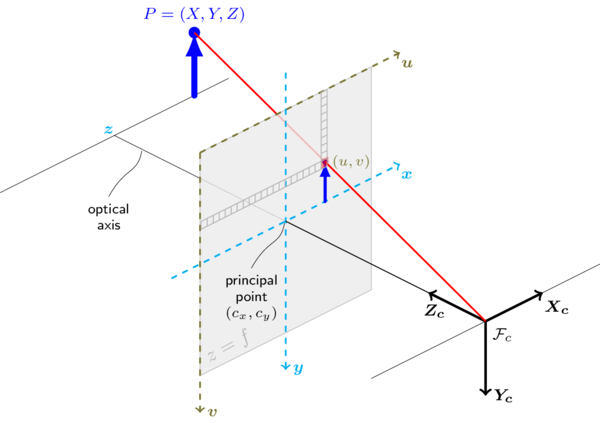
\includegraphics[width=.75\columnwidth]{pinhole.png}
\caption{Modelo de Câmera Estenopeica\cite{docsopencv}}
\end{center}
\end{figure}

Se os pontos do mundo \(X\) e da imagem \(x\) são representados por coordenadas homogêneas, podemos expressar matematicamente a projeção da câmera como uma matriz\cite{tese}:

\begin{equation}\lambda  x = P  X\end{equation}

onde \(\lambda\) é um fator de escala e P é a matriz 3x4 de projeção, também chamada matriz de calibração.

P pode ser decomposta em duas entidades geométricas: os parâmetros intrísecos \(K\) e extrínsecos \(R\) e \(t\) de calibração\cite{tese}
\begin{equation}
P = K [R | t]
\end{equation}
\begin{equation}
t = -R\widetilde{C}
\end{equation}
onde \(\widetilde{C}\) é a origem do sistema de coordenadas da câmera\cite{Hartley2004}.

Os parâmetros intrísecos de calibração descrevem a transformação entre a imagem ideal e a imagem em pixels
\begin{equation}
K = \begin{pmatrix} 
f & s & c_x \\
0 & \alpha f & c_y\\
0 & 0 & 1
\end{pmatrix}
\end{equation}
e os extrínsecos são a rotação \(R\) e translação \(t\) que transformam pontos no espaço do objeto para pontos no espaço da imagem\cite{tese}.

Como há 6 graus de liberdade nos parâmetros extrínsecos e 5 nos intrísecos, é necessário pelo menos 6 correspondências \({x_i \leftrightarrow X_i}\) do mesmo ponto no espaço da imagem e no espaço do objeto para obter P\cite{tese}. Mas dado que há um erro inerente nas medidas experimentais, para melhorar a qualidade da estimativa é preciso usar \(n > 6\) correspondências (como será visto em \ref{metodologia}, usaremos 48 pontos) e, assim, não há uma única matriz P que satisfaz esse sistema de equações. Precisamos, portanto, adicionar restrições para encontrar uma solução única.  

Um método comum é adicionar a restrição \(p_{34} = 0\)\cite{Hartley2004}, mas uma melhor abordagem\cite{tese} é:

\begin{equation}
\begin{aligned}
P = \min_{P'} \sum_{i}d(x_i, P'Xi)^2
\end{aligned}
\end{equation}
onde \(d(x_i, P'Xi) \) é a distância euclidiana entre o ponto observado e o estimado. 

\subsection{Distorções}

O modelo até aqui descrito descreve uma câmera ideal, mas as lentes das câmeras reais podem gerar distorções, que também são parâmetros intrínsecos que precisam ser considerados. 

A distorção radial é a mais importante e causa uma curvatura no mapeamento.

\begin{figure}[ht!]
\begin{center}
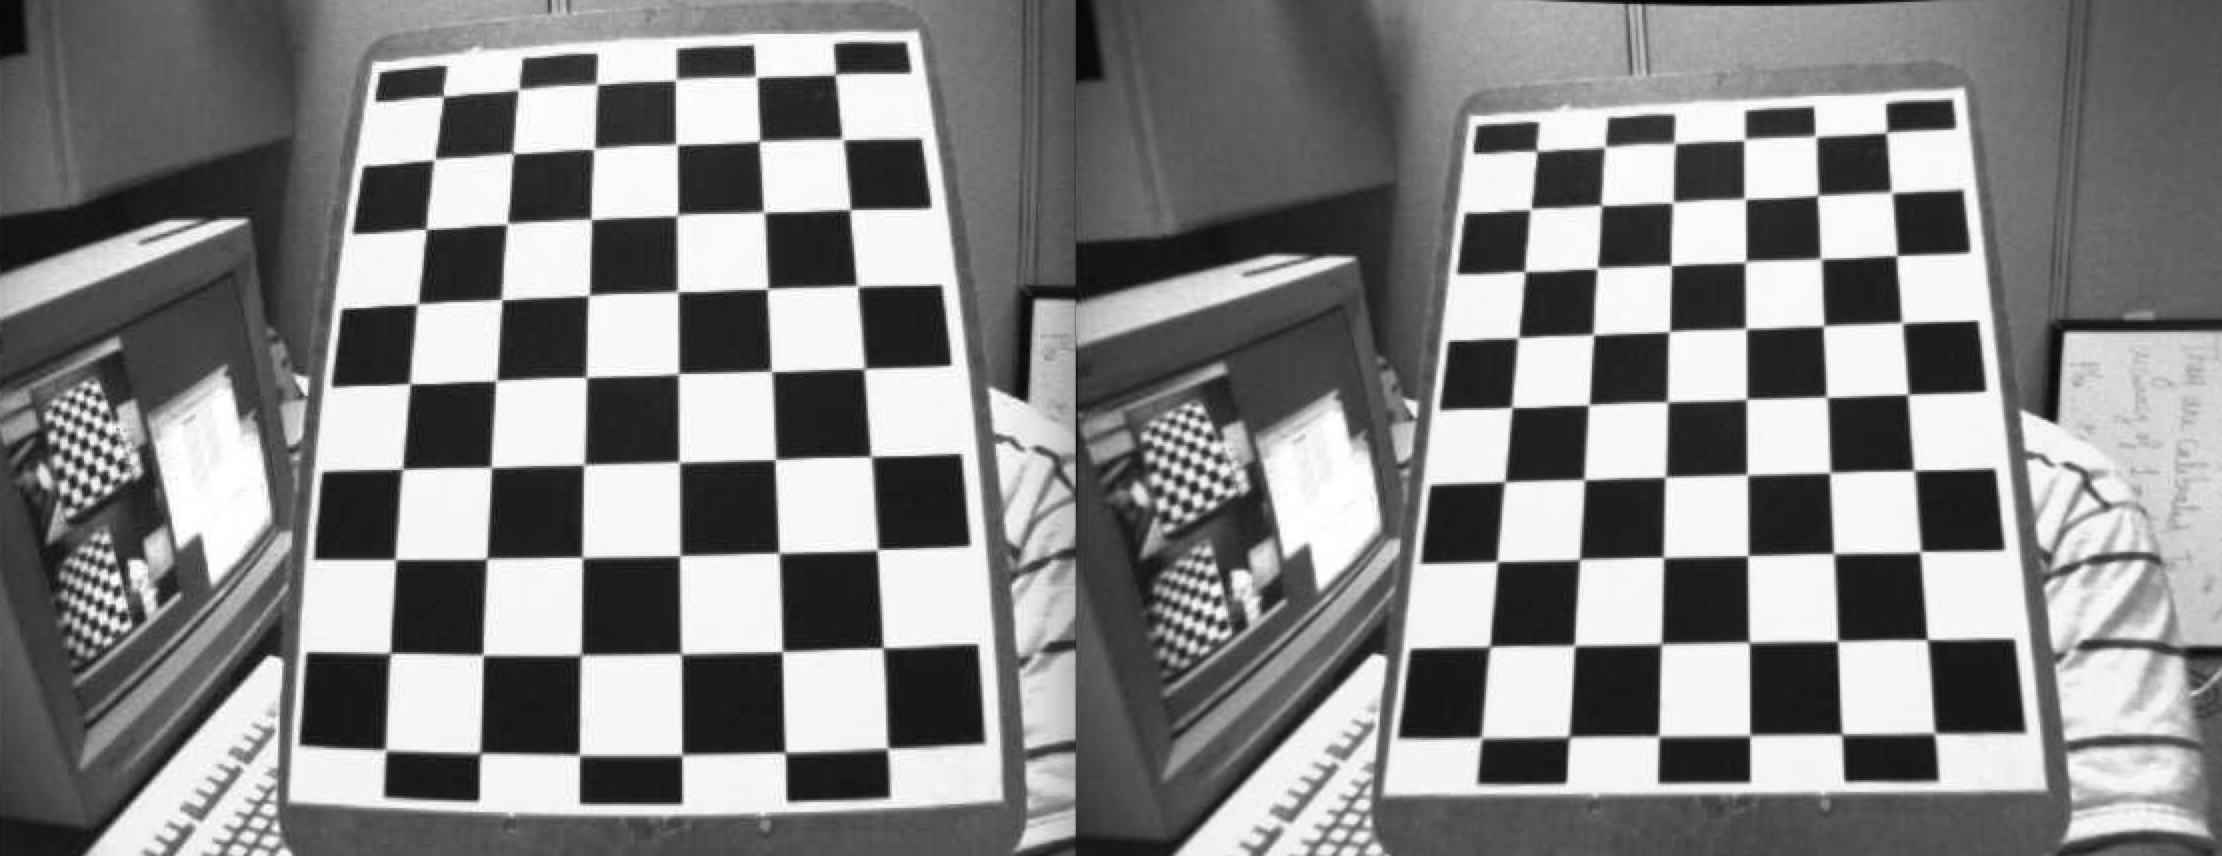
\includegraphics[width=\columnwidth]{distortion.png}
\caption{Distorção Radial\cite{docsopencv}}
\end{center}
\end{figure}

A correção dessa distorção pode ser modelada da seguinte maneira\cite{docsopencv}: 

    \[x_{retificado} = x( 1 + k_1 r^2 + k_2 r^4 + k_3 r^6)\]
    \[y_{retificado} = y( 1 + k_1 r^2 + k_2 r^4 + k_3 r^6)\]

Outra distorção comum é a tangencial, que ocorre quando o plano da lente não está alinhado. Para corrigir:


\[x_{retificado} = x + [ 2p_1xy + p_2(r^2+2x^2)] \]
\[y_{retificado} = y + [ p_1(r^2+ 2y^2)+ 2p_2xy] \]


Esses cinco parâmetros são conhecidos como coeficientes de distorção
\((k_1 \hspace{10pt} k_2 \hspace{10pt} p_1 \hspace{10pt} p_2 \hspace{10pt} k_3)\)\cite{docsopencv}.

\section{Metodologia}\label{metodologia}
O modelo da câmera e seus parâmetros foram descritos na seção de Revisão Teórica. Nesta seção, descreve-se como estimá-los experimentalmente.

\subsection{Materiais}
Foram utilizados:
\begin{itemize}
\item uma tábua de compensado
\item papel contact
\item fita adesiva
\item um padrão de calibração xadrez impresso em papel A4
\item uma trena
\item uma régua
\item computador MacBook Pro (Retina, 13-inch, Early 2015), Processador Intel Core i5 2,7 GHz, 8GB de RAM
\item Python 3.6.3 :: Anaconda custom (64-bit)
\item OpenCV 3.4.0
\item sete programas em python especialmente desenvolvidos para o projeto. Todos estão disponíveis no repositório: \url{git@github.com:fredguth/unb-cv-3183.git}\label{repo}
\end{itemize}

\subsection{Preparação}
 \begin{enumerate}
 \item Imprime-se o padrão de calibração em folha A4 e o cola à tábua de compensado usando o Papel Contact.
 \item Com o programa \textit{requisito1.py}, abre-se uma imagem jpg e com cliques do mouse desenha-se um segmento de reta sobre a imagem entre o primeiro e o segundo clique, registrando-se a distância \(||p2 - p1||_2 \) na própria imagem aberta. 
 \end{enumerate}
\subsection{Obtenção dos parâmetros intrínsecos}
 \begin{enumerate}
  \item Executa-se o programa \textit{requisito2.capture.py} que abre um stream de vídeo e grava a imagem sempre que detecta os cantos dos quadrados no padrão de calibração de tabuleiro de xadrez. O programa pede o número do experimento e grava as imagens capturadas no diretório do mesmo.  Foram feitos 8 experimentos que geraram entre 25 e 70 imagens cada.
  \item Executa-se o programa \textit{requisito2.calibrate.py} para cada experimento. O programa detecta os cantos dos quadrados do padrão de calibração xadrez e refina essa detecção para obter os parâmetros intrínsecos K e os coeficientes de distorção. É importante mover o quadrado no campo de captura da câmera em diversas orientações e posições, em diferentes distâncias. Os parâmetros intrínsecos e coeficientes de distorção são automaticamente armazenados em arquivos xml nos diretórios dos respectivos experimentos.
\item Dado que já temos os coeficientes de distorção, com o programa \textit{requisito2.measure.py} retificamos as imagens da câmera e permitimos medir distâncias na imagem retificada em pixels. 
\item Após todos os experimentos executados, executa-se o programa \textit{requisito2.analyse.py} que gera a média e o desvio parão dos parâmetros intrísecos, salvando-os no diretório \textit{exp-0}.
\end{enumerate}
\subsection{Obtenção dos parâmetros extrínsecos}\label{extrinsecos}
\begin{enumerate}
\item Com a régua, mede-se o tamanho de um quadrado no padrão de calibração.
\item Executa-se o programa \textit{requisito3.py}, que computa a correspondencia entre pontos da imagem e do espaço do objeto, atribuindo como origem do sistema de coordenadas do mundo, o ponto de intersecção do canto superior esquerdo do tabuleiro e através da função \textit{solvePnP} da OpenCV\cite{OpenCV}, obtem os parâmetros extrínsecos R e t. 
\item Quando o programa pede o número do experimento, escolhe-se \(0\), uma vez que queremos usar os parâmetros intrísecos médios, medidos na etapa anterior.

\item Deixa-se a câmera em um ponto marcado pela fita adesiva, tentando colocá-la ortogonal ao plano da sua base. 
\item Com a câmera posicionada, posiciona-se o tabuleiro na distância mais próxima possível da câmera em que o padrão de calibração tem seus cantos detectados (os cantos ficam marcados com pontos coloridos no \textit{stream} da câmera), marcando com a fita adesiva este ponto como \(d_{min}\). \label{montagem}
\item Repete-se o passo anterior, tentando encontrar a distância mais afastada da câmera. Marca-se este ponto com fita adesiva como \(d_{max}\); e também um ponto intermediário entre \(d_{min}\) e \(d_{max}\), que chamamos \(d_{med}\).
\item Medimos as distâncias \(d_{min}\), \(d_{med}\)  e \(d_{max}\) com a trena.
\item Com todos os pontos marcados e a câmera posicionada, acionamos o modo de captura apertando a tecla \textit{espaço}
\item Leva-se o tabuleiro de xadrez para \(d_{min}\) e após algumas capturas (identificação do padrão xadrez na imagem \textit{stream} da câmera), apertamos a tecla \textit{espaço} novamente para sair do modo captura.\label{medicao}
\item Repete-se os últimos dois passos para as distâncias \(d_{med}\) e \(d_{med}\). As imagens captadas com as respectivas distâncias medidas são gravadas no diretório do experimento selecionado. É importante verificar se há pelo menos 3 imagens gravadas para cada distância.
\end{enumerate}
\subsection{Obtenção da altura de um objeto através da sua imagem}
Com os parâmetros intrínsecos e extrínsecos,  é possível medir um objeto no mundo real a partir da sua imagem. Neste projeto, entretanto, não se obteve êxito em desenvolver essa funcionalidade no programa \textit{requisito4.py}

\section{Resultados}
Nesta seção apresentamos, para cada etapa da \ref{metodologia}, os resultados obtidos. Todos os dados podem ser acessados no repositório do projeto (\ref{repo}).
\subsection{Medição em pixels de segmentos de imagens}
\begin{figure}[ht!]\label{baboon}
\begin{center}
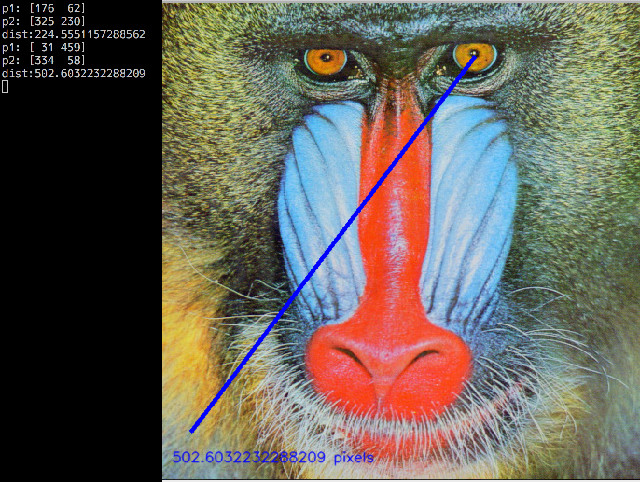
\includegraphics[width= .5\columnwidth]{baboon.jpg}
\caption{Medição em pixels de segmentos em imagens}
\end{center}
\end{figure}
A figura \ref{baboon} mostra a medição em pixels de segmentos entre cliques na imagem. Além da saída no \textit{console}, o programa mostra a distância em pixels na própria tela.
\subsection{Calibração dos parâmetros intrínsecos}

A figura \ref{snapshots} mostra diversas das imagens captadas para calibração, onde tentou-se explorar ao máximo a diferença de posição, distância e até luminosidade do ambiente.
\begin{figure}[!htb]\label{snapshots}
\minipage{0.33\columnwidth}
  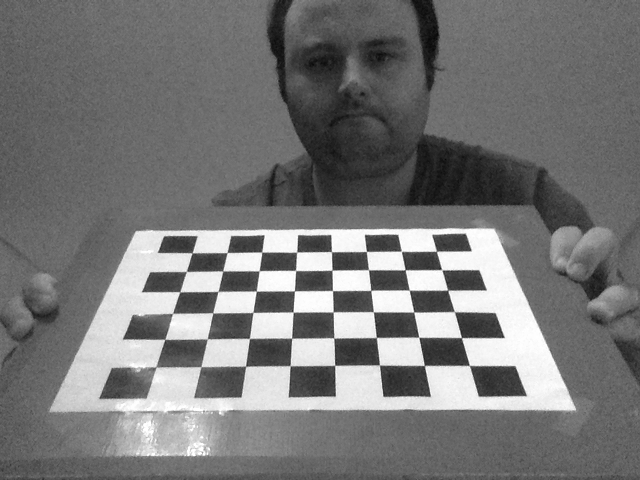
\includegraphics[width=\linewidth]{snap-1.png}
\endminipage\hfill
\minipage{0.33\columnwidth}
  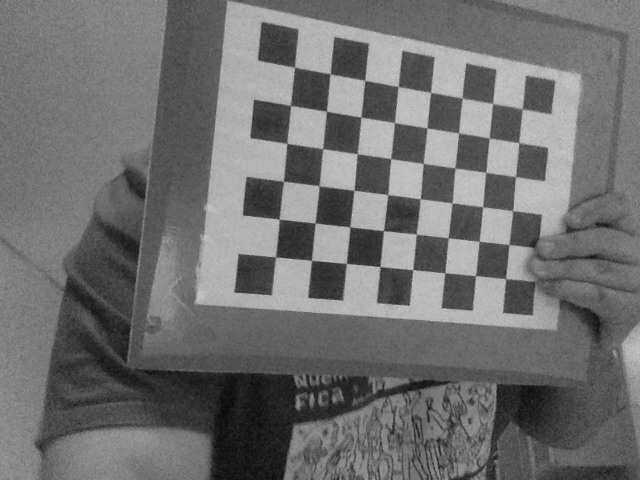
\includegraphics[width=\linewidth]{snap-2.png}
\endminipage\hfill
\minipage{0.33\columnwidth}%
  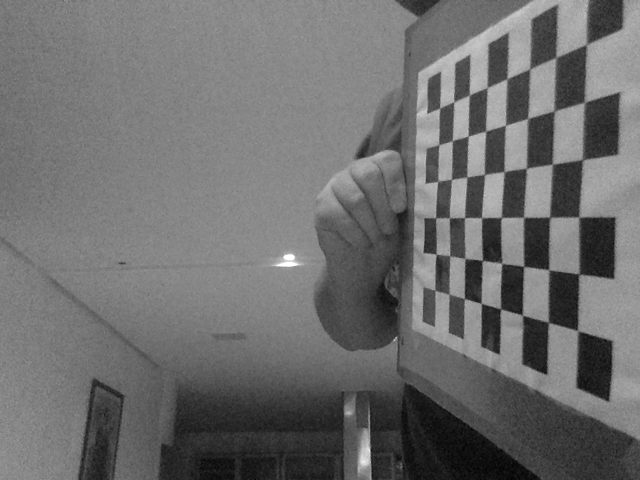
\includegraphics[width=\linewidth]{snap-3.png}
\endminipage\hfill
\minipage{0.33\columnwidth}
  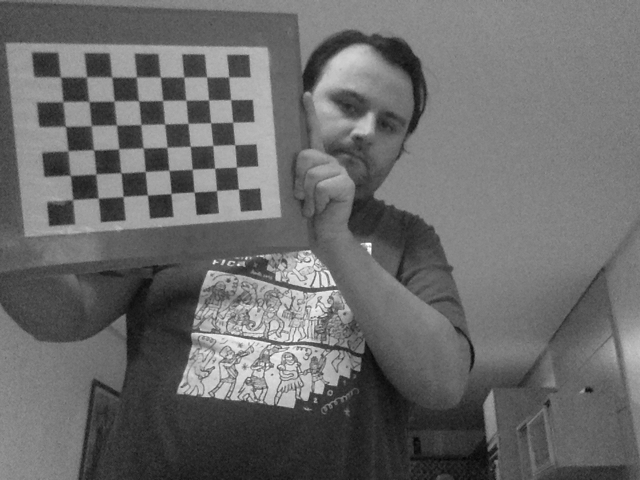
\includegraphics[width=\linewidth]{snap-4.png}
\endminipage\hfill
\minipage{0.33\columnwidth}
  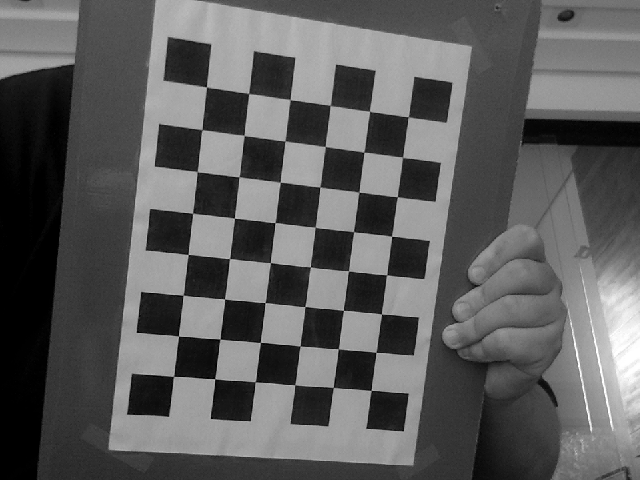
\includegraphics[width=\linewidth]{snap-5.png}
\endminipage\hfill
\minipage{0.33\columnwidth}%
  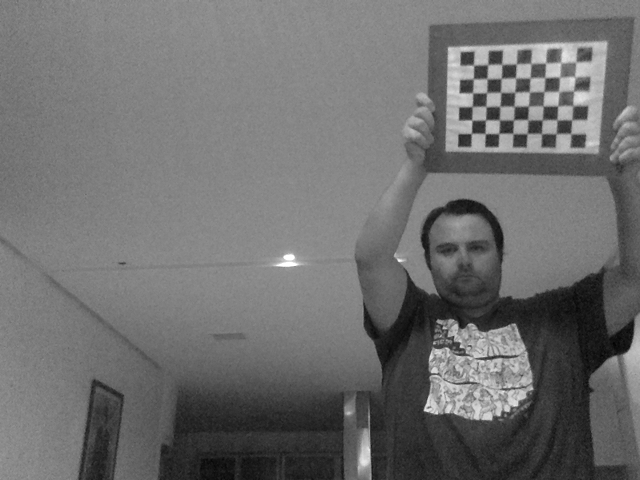
\includegraphics[width=\linewidth]{snap-6.png}
\endminipage\hfill
\caption{Algumas das dezenas de \textit{snapshots} geradas em diferentes posições}
\end{figure}
O resultado obtido para os parâmetros intrínsecos foram:
$$
K = \begin{pmatrix} 
673.08 & 0 & 312.32 \\
0 & 668.10 & 236.50\\
0 & 0 & 1
\end{pmatrix}
\pm
\begin{pmatrix} 
56.27 & 0 & 13.24 \\
0 & 55.75 & 22.71\\
0 & 0 & 1
\end{pmatrix}
$$
\((k_1=0.150\pm0.039 \hspace{10pt} k_2=-.744\pm0.448 \hspace{10pt} p_1=0.003\pm0.003 \hspace{10pt} p_2=-0.003\pm0.007 \hspace{10pt} k_3=1.820\pm1.932)\)
\subsection{Calibração dos parâmetros extrínsecos}\label{calibextr}
Na figura \ref{extr} mostramos como foram capturadas as imagens para obtenção dos parâmetros extrínsecos.
\begin{figure}\label{extr}
\centering
\begin{minipage}{.45\columnwidth}
  \centering
  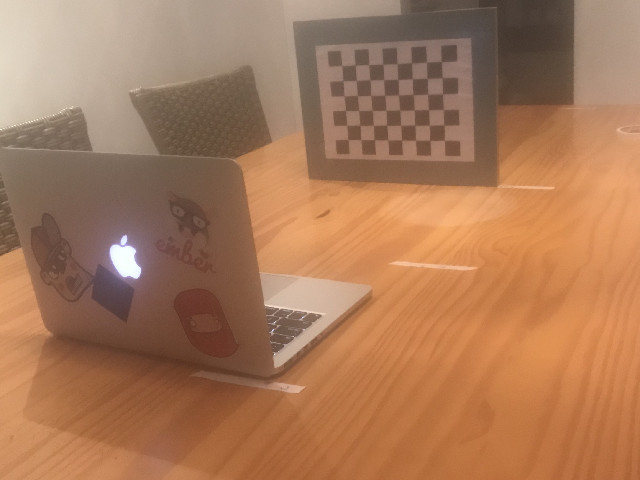
\includegraphics[width=.95\linewidth]{cena.jpg}
  \caption{Montagem \ref{extrinsecos}.\ref{montagem}}
  \label{fig:test1}
\end{minipage}%
\begin{minipage}{.45\columnwidth}
  \centering
  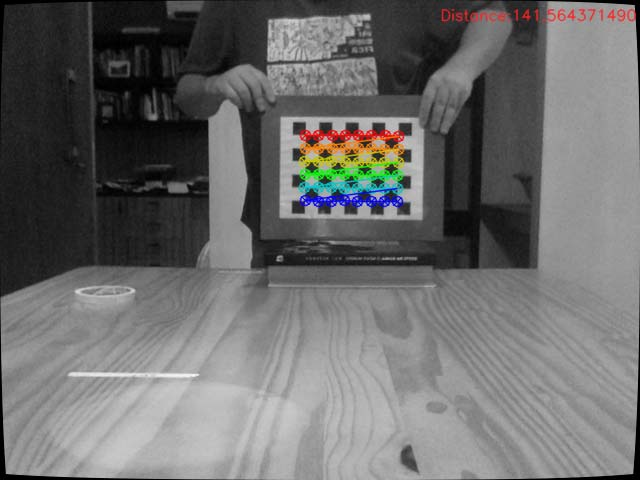
\includegraphics[width=.95\linewidth]{extr.jpg}
  \caption{Medição \ref{extrinsecos}.\ref{medicao}}
  \label{fig:test2}
\end{minipage}
\end{figure}
O resultado está apresentado na tabela \ref{distancias}.
\begin{table}[htbp]\label{distancias}
\caption{Comparação distâncias estimadas versus real}
\begin{center}
\begin{tabular}{|c|c|c|c|c|c|c|}
\hline
em \textit{cm}& \textbf{\textit{Real}}& \(d_{1}\)&\(d_{1}\)&\(d_{3}\)&\(\bar{d}\)& \textbf{\(\sigma\)} \\
\hline
\(d_{min}\)& 32.3& 31.35& 31.93 & 31.97& 31.75& 0.35\\
\hline
\(d_{med}\)& 72.3& 69.51& 68.87 & 68.57& 68.98& 0.48\\
\hline
\(d_{max}\)& 148.1& 138.78& 141.87 & 144.31& 141.65& 2.77\\
\hline

\end{tabular}
\label{tab1}
\end{center}
\end{table}
O erro ficou entre 2 e 6\%. Um pouco acima da margem de 2\% do desvio padrão.
\subsection{Medição de Objeto 3D a partir de sua imagem}
\section{Discussão e Conclusões}
Neste trabalho, utilizamos o modelo de câmera estenopeica para fazer mapeamentos de posições no mundo real para a imagem e vise-versa. O resultado obtido para as distâncias \ref{calibextr} na calibração dos parâmetros extrínsecos tiveram um erro menor do que 6\%. Entretanto, cabe ressaltar que para isso foi necessário capturar centenas de imagens na fase de calibração dos intrínsecos. Tentativas feitas que usavam poucas dezenas não lograram êxito. 

% \begin{figure}[htbp]
% \centerline{
\includegraphics{fig.jpg}}
% \caption{Example of a figure caption.}
% \label{fig}
% \end{figure}

\selectlanguage{brazilian}
\bibliographystyle{IEEEtran}
\bibliography{references}

\end{document}
